\documentclass[11pt]{article}

% --- Page layout ---
\usepackage[a4paper,margin=2cm]{geometry}   % A4 paper with 2cm margins
\usepackage{multicol}                       % Support for multiple columns
\setlength{\columnsep}{1cm}                % Space between columns
\setlength{\columnseprule}{0.4pt}          % Vertical line between columns

% --- Typography and section formatting ---
\usepackage{titlesec}                       % Custom section title formatting
\titleformat{\section}{\normalfont\Large\bfseries}{}{0pt}{} % Section format
\titleformat{\subsection}{\normalfont\large\bfseries}{}{0pt}{} % Subsection format
\usepackage{parskip}                        % Adds space between paragraphs, no indent

% --- Lists and boxes ---
\usepackage{enumitem}                       % Customise list spacing and bullets
\usepackage[most]{tcolorbox}               % Nice boxes (e.g., for Executive Summary)
\tcbset{
	colback=blue!5,       % Light blue background
	colframe=black,       % Border color
	boxrule=0.5pt,        % Border thickness
	arc=1mm,              % Rounded corners
	left=6pt, right=6pt, top=6pt, bottom=6pt  % Padding
}

% --- Figures and tables ---
\usepackage{graphicx}                       % Insert images
\usepackage{float}                          % [H] float positioning
\usepackage{booktabs}                       % Nicer tables
\usepackage{caption}                        % Custom caption formatting
\captionsetup[figure]{justification=centering} % Center figure captions

% --- END of preamble ---

\begin{document}
	
	\begin{center}
		\LARGE\textbf{Policy Brief: Does High Homeownership Raise Youth Unemployment in Europe?}
	\end{center}
	
	\begin{multicols}{2}
		
		\section*{Executive Summary}
		
		\vspace{-1em}
		
		\begin{tcolorbox}
			\begin{itemize}[left=0.3em, labelsep=0.5em, labelwidth=0.6em, itemsep=0pt, topsep=0pt]
				\item In 2011, youth unemployment and homeownership rates showed a \textbf{moderate positive correlation} (\textit{r = 0.57}).
				\item By 2018, this relationship had \textbf{weakened considerably} and was \textbf{no longer statistically significant} (\textit{r = 0.16}).
				\item Panel regression models show that \textbf{lagged homeownership} has a \textbf{small but significant effect} (\textit{Coef: 0.027}) on higher youth unemployment, even after controlling for year and country factors.
				\item \textbf{Lagged age structure} and \textbf{tertiary education} are statistically insignificant and contribute minimally to the model.
				\item While countries like \textbf{Greece}, \textbf{Spain}, and \textbf{Italy} display both \textbf{high homeownership} and \textbf{high youth unemployment}, others like \textbf{Ireland} and \textbf{Norway} stand out as outliers, with \textbf{high ownership} and \textbf{low youth unemployment}.
			\end{itemize}
		\end{tcolorbox}
		
		\vspace{-1em}
		
		\section*{Background and Context}
		\indent In recent decades, governments across the Global North have actively promoted homeownership as a route to wealth accumulation, stable communities, and civic participation. However, a growing body of research highlights potential labour market downsides of this policy emphasis. Blanchflower and Oswald (2013) argue that high ownership can increase unemployment by \textit{reducing geographic mobility}, \textit{increasing commuting distances}, and \textit{discouraging new business formation}. These mechanisms may be particularly relevant for young people (aged 16-24) who tend to face more precarious labour market conditions and rely more heavily on spatial mobility to access job opportunities.
				
		\vspace{-1em}
		
		\section*{Data and Methods}
		\indent We analyse Eurostat data for 29 European countries (2011-2018), focusing on youth unemployment (aged 16-24) and homeownership rates. We explore the evolving relationship between the two over the study period using scatterplots and Pearson's correlations. To normalise skewness, we log-transform youth unemployment and use lagged homeownership as the key predictor. Fixed-effects regressions control for year and country differences, isolating the effect of homeownership. Demographic factors were tested but did not meaningfully improve model fit and were excluded from the final specification.
		
		\vspace{-1em}
		
		\section*{Key Findings}
		
		\subsection*{Descriptive Trends}
		\indent In 2011, countries with higher homeownership generally had higher youth unemployment. This relationship is visually evident in Figure~. Spain, Greece, and Latvia are clear drivers of the trend. However, by 2018, this relationship becomes flat, as shown in Figure
		
		\begin{figure}[H]
			\centering
			\caption{Youth Unemployment 2011}
			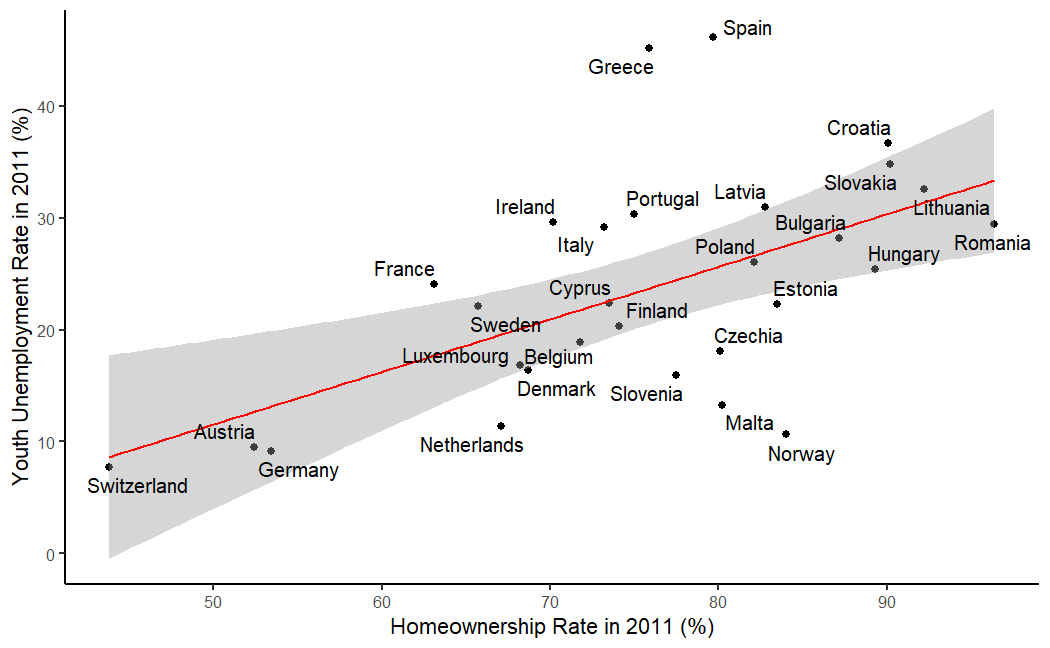
\includegraphics[width=1\linewidth]{youth_unemployment_2011.png}
			\label{fig:youth_unemployment_2011}
		\end{figure}
		
		\vspace{-1em}
		
		\begin{figure}[H]
			\centering
			\caption{Correlation Over Time (2012-2018)}
			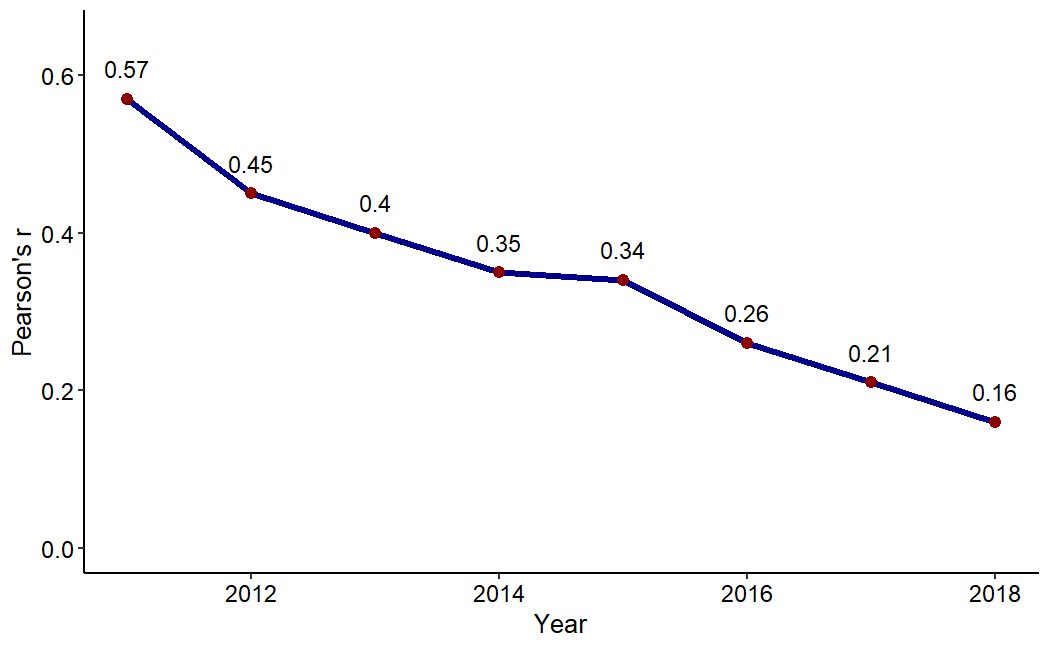
\includegraphics[width=1\linewidth]{cor_year.png}
			\label{fig:cor_year}
		\end{figure}
		
		\vspace{-1em}
		
		\begin{figure}[H]
			\centering
			\caption{Youth Unemployment Trends}
			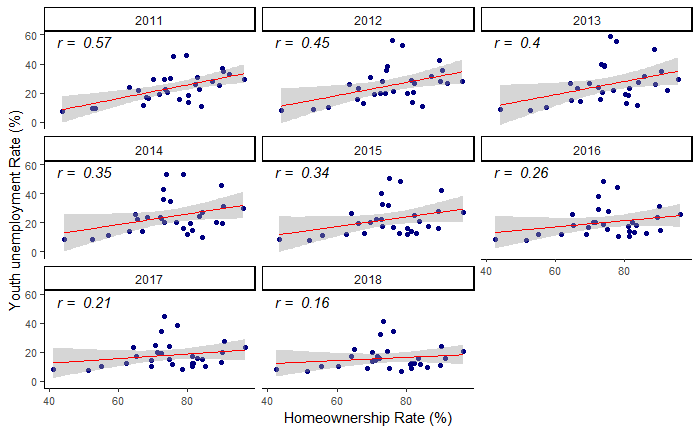
\includegraphics[width=1\linewidth]{youth_unemployment_trends.png}
			\label{fig:youth_unemployment_trends}
		\end{figure}
		
		\begin{figure}[H]
			\centering
			\caption{Change in Homeownership}
			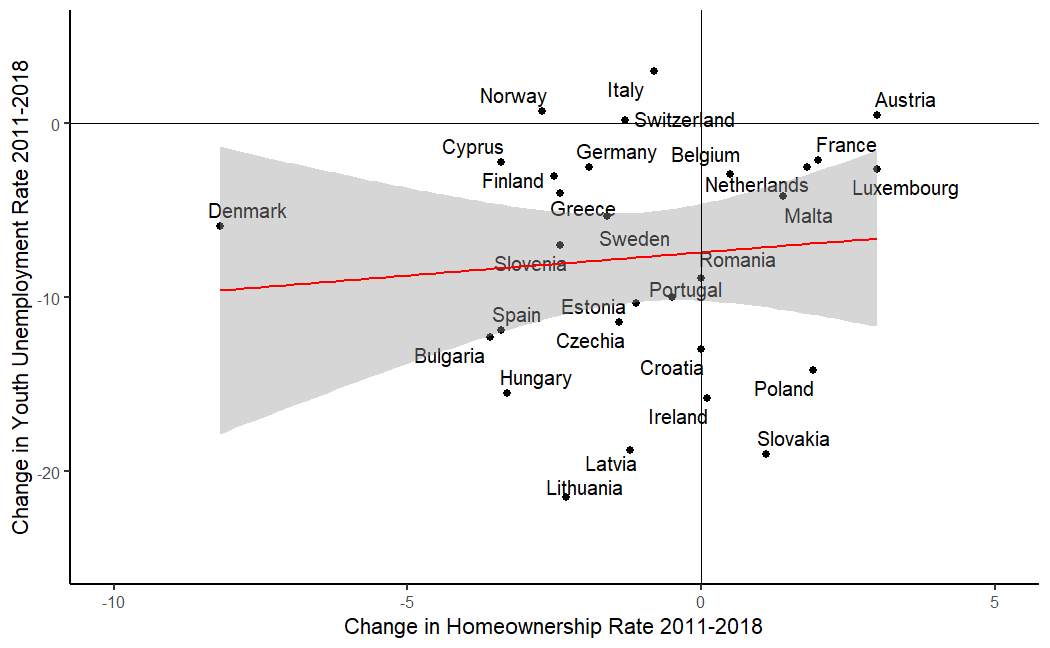
\includegraphics[width=1\linewidth]{change_homeownership_7years.png}
			\label{fig:change_homeownership_7years}
		\end{figure}
		\vspace{-1em}
		
		\subsection*{Regression Models}
		\indent Table~ presents fixed-effects models predicting logged youth unemployment. Model 1 uses only lagged homeownership; Model 2 adds controls for age and education; Models 3 and 4 add year and country dummies.
		
		\begin{table}[H] \centering 
			\caption{} 
			\label{} 
			\small
			\begin{tabular}{@{\extracolsep{5pt}}lc} 
				\\[-1.8ex]\hline 
				\hline \\[-1.8ex] 
				& \multicolumn{1}{c}{\textit{Dependent variable:}} \\ 
				\cline{2-2} 
				\\[-1.8ex] & Log\_youthunemp \\ 
				\hline \\[-1.8ex] 
				Lag\_own & 0.016$^{***}$ \\ 
				& (0.003) \\ 
				& \\ 
				Constant & 1.699$^{***}$ \\ 
				& (0.216) \\ 
				& \\ 
				\hline \\[-1.8ex] 
				Observations & 196 \\ 
				R$^{2}$ & 0.145 \\ 
				Adjusted R$^{2}$ & 0.141 \\ 
				Residual Std. Error & 0.467 (df = 194) \\ 
				F Statistic & 32.895$^{***}$ (df = 1; 194) \\ 
				\hline 
				\hline \\[-1.8ex] 
				\textit{Note:}  & \multicolumn{1}{r}{$^{*}$p$<$0.1; $^{**}$p$<$0.05; $^{***}$p$<$0.01} \\ 
			\end{tabular} 
		\end{table} 
		
		\vspace{-1em}
		
		\section*{Policy Implications}
		\indent Youth unemployment appears to be modestly affected by prior-year homeownership rates. Policies that encourage labour mobility (e.g. flexible housing markets, rental support, and transport subsidies) may help mitigate immobility effects. Given the decline in correlation after 2015, structural labour market recovery likely dampened the homeownership-unemployment link. However, in some Southern European countries, persistent housing tenure rigidity may still constrain young people's employment prospects.
		
		\vspace{-1em}
		
		\section*{Recommendations}
		\begin{itemize}[left=1em, itemsep=0pt]
			\item \textbf{Avoid policies that over-prioritise homeownership} for youth; increase access to affordable rental housing.
			\item \textbf{Target labour mobility} through transport infrastructure and relocation grants.
			\item \textbf{Monitor tenure and employment jointly}, particularly in laggard regions.
			\item \textbf{Account for local context}: in countries with weak youth employment but high ownership (e.g. Italy, Greece), housing reform could play a critical role.
		\end{itemize}
		
		\vspace{-1em}
		
		\section*{Limitations}
		\indent This brief uses national-level panel data and does not model potential spatial spillovers or family dynamics. Youth unemployment may also be driven by sectoral or educational mismatches not captured in the dataset. Finally, results are correlational; causal inference requires further study.
		
		\section*{Conclusion}
		\indent While Oswald and Blanchflower's thesis finds partial support in the youth labour market, the effect of homeownership has diminished over time. Still, policy should remain attentive to how housing systems structure opportunities for youth in the European labour market.
		
	\end{multicols}
\end{document}